\newpage
\section{Heuristics approaches for pairwise sequence alignment}
These methods are very popular because they are much faster than dynamic
programming and at the same time they return excellent alignment of biological
sequences.

\paragraph*{From Wikipedia}
Word methods, also known as k-tuple methods, are heuristic
methods that are not guaranteed to find an optimal alignment solution,
but are  significantly more efficient than dynamic programming.

These methods are especially useful in large-scale database searches where
it is known that a large proportion of the candidate sequences will
have essentially no significant match with the query sequence.

Word methods are best known for their implementation in the database
search tools \textbf{FASTA and the BLAST} family.

\subsection{General strategy}

Let $A$ and $B$ be two sequence to be aligned. The general strategy of these
methods is based on two main steps:

\begin{enumerate}
  \item Produce a \textbf{lookup table} where the words of length $k$
($k$-mers) present in sequence $A$ are indexed, including all the positions
where they occur in sequence $A$.
  \item Read sequence $B$, word by word. For every word check in the lookup
talbe if and where the word occur in sequence $A$. Then try to extend the
alignment.
\end{enumerate}

Other strategies are: FASTA, BLAST and BLAT.

\paragraph*{Conversion of DNA $k$-mers into numbers}

Any word can be easily translated into an integer number.
DNA has an alphabet of 4 symbols, thus the number of possible words will be
$4^k$ where $k$ is the word length.

Every symbol is associated to a value: for DNA, in binary notation
generally is $A=00,\ C=01,\ G=10,\ T=11$. The translation of a word into a
number is therefore very fast.

The resulting number can be directly used as an index to point
to the address with the information about that word (i.e. all the positions
where it occurs).

With a given DNA you can translate the four DNA symbols A, C, G, T with a
binary number (see above).

In this way you can convert a DNA sequence into a number.
This can be done also with amino acids.

\subsection{FASTA}

The FASTA programs find regions of local or global similarity between
proteins or DNA sequences, either by searching proteins or DNA databases, or by
identifying local duplications within a sequence.

Other programs provide information on the statistical significance of an
alignment.

Like BLAST, FASTA can be used to infer functional and evolutionary relationships
between sequences as well as help identify members of gene families.

Imagine a sequence placed at the top and a sequence placed on the left side,
both starting at the top left corner.

The sequence at the top is indexed, memorizing all the occurrences and
position of each kmer.

Then the sequence at the left is read, one kmer at a time.
All the ``growing'' diagonals are memorized to produce the result shown
in panel A (figure \ref{fig:fasta}).

Even if you have kmer of length one ($ktup = 1$), you will find better
performance compared to Smith \& Waterman. This because you have to do less
operation with FASTA.

Smith \& Waterman algorithm should be used only if you go for a full match.
Analyzing a full alignment is expensive but with Smith \& Waterman
is very accurate.

\begin{figure}[H]
  \centering
  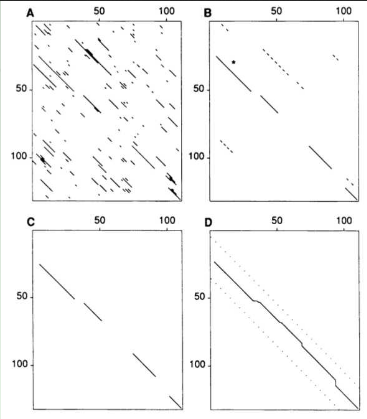
\includegraphics[scale=0.5]{FASTA}
  \caption{FASTA}
  \label{fig:fasta}
\end{figure}

\textbf{Question}: If I have a very long sequence and several short DNA
sequence, is it better to index the long or the short sequence? \\

\textbf{Answer}: It's better to index the long sequence, because you can
check all the differents sequences in the database where are all the data are
present.

\subsection{BLAST}

Blast is probably the most popular program for the alignment of biological
sequences.

As FASTA, BLAST uses a lookup table, but it creates also an index for the
similarities with a given threshold. Another difference from FASTA is that
BLAST tries to extend locally each ``seed'', to obtain a high-scoring segment
pair.

\begin{figure}[H]
  \centering
  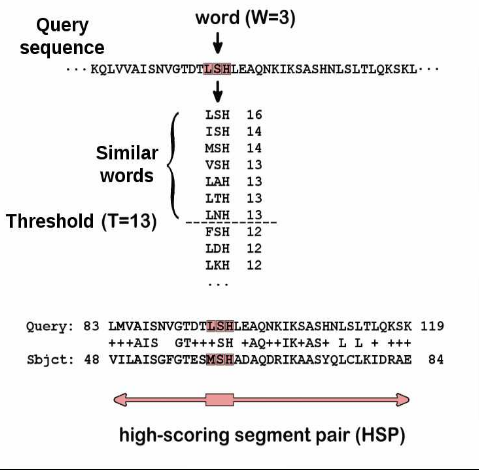
\includegraphics[scale=0.5]{BLAST}
  \label{fig:blast}
\end{figure}

BLAST is a little faster than FASTA. Most people use BLAST also for DNA
alignment and it works well.

Different flavours of BLAST:
\begin{itemize}
  \item Nucleotide blast
  \item Protein blast
  \item blastx
  \item tblastn
  \item tblastx
\end{itemize}

%exam question
\textbf{Question}: What's the meaning of translate the sequence in proteins? \\

\textbf{Answer}: If you consider evolution of sequences, the natural selection
is keepeng some of this information working and very often this natual
selection is working at the protein level.
Sometimes you can have 2 nucleotide sequences completely different that
encode the same protein, so it's much more accurate do it at the protein level.

\subsection{BLAT}

BLAT is an alignment tool like BLAST, but it's structured differently. On DNA,
BLAT works by keeping an index of an entire genome in memory.

The best things to do it's to align RNA with Genom.

New version of BLAT can index more kmer.
